\section{Численный метод}
\subsection{Общая идея сеточно-характеристического метода}
\subsubsection{Расщепление по направлениям}

Сведём решение исходной системы в трёхмереном пространстве
\begin{equation}
	\label{matrix_anisotropy_equation1}
	\frac{\partial\vec{u}}{\partial{t}}+\mathbf{A}_x\frac{\partial\vec{u}}{\partial{x}}+
	\mathbf{A}_y\frac{\partial\vec{u}}{\partial{y}}+
	\mathbf{A}_z\frac{\partial\vec{u}}{\partial{z}}=0
\end{equation}
к решению одномерной системы:
\begin{equation}
	\label{norm_form}
	\frac{\partial\vec{u}}{\partial{t}}+\mathbf{A_i}\frac{\partial\vec{u}}{\partial{x_i}} = 0.
\end{equation}

Обозначим оператор $f_i$ как переход с одного временного слоя на другой при численном решении уравнения \eqref{norm_form}:
\begin{equation}
	\label{simple_splitting}
	\vec{u_i}^{n} = f_i(\mathbf{A}_i)\vec{u}^{n},
\end{equation}
а оператор $F$ -- как такой переход для трёхмерного уравнения. Тогда \cite{chelnokov} будет верно с первым порядком точности по времени:
\begin{eqnarray}
\label{simple_3D_split_operator}
F = \alpha_0 f_0(\frac{\mathbf{A}_0}{\alpha_0}) + \alpha_1 f_1(\frac{\mathbf{A}_1}{\alpha_1}) + \alpha_2 f_2(\frac{\mathbf{A}_2}{\alpha_2}), \\
\alpha_0 + \alpha_1 + \alpha_2 = 1,
\end{eqnarray}
и со вторым поряком точности по времени:
\begin{equation}
\label{3D_split_operator}
F = \frac{1}{6}\sum_{i \neq j \neq k \neq i} f_i(\mathbf{A}_i)f_j(\mathbf{A}_j)f_k(\mathbf{A}_k).
\end{equation}

Вычисление по схеме \eqref{3D_split_operator} слишком затратны по количеству вычислений и памяти. Однако, как показывает практика, с достаточной точностью работает следующее к ней приближение:
\begin{equation}
\label{short_3D_split_operator}
F = f_0(\mathbf{A}_0)f_1(\mathbf{A}_1)f_2(\mathbf{A}_2),
\end{equation}
которое является первым слагаемым в \eqref{3D_split_operator}. Такое приближение обладает тем достоинством, что оно не только близко ко второму порядку, но и экономичнее по памяти, чем \eqref{simple_3D_split_operator}.

\subsubsection{Сеточно-характеристический метод в одномерном случае}
Из гиперболичности рассматриваемой системы уравнений следует диагонализуемость матриц $\mathbf{A}_i$:
\begin{equation}
	\label{diagonal_view}
	\mathbf{A} = \mathbf{\Omega}^{-1}\mathbf{\Lambda}\mathbf{\Omega}.
\end{equation}	
Умножим \eqref{norm_form} справа на $\mathbf{\Omega}$:
\begin{equation}
	\label{norm_form1}
	\mathbf{\Omega}\frac{\partial\vec{u}}{\partial{t}}+\mathbf{\Lambda}\mathbf{\Omega}\frac{\partial\vec{u}}{\partial{x}} = 0.
\end{equation}
В приближении локальной однородности среды можно внести $\mathbf{\Omega}$ под знак дифференциала:
\begin{equation}
	\label{norm_form2}
	\frac{\partial(\mathbf{\Omega}\vec{u})}{\partial{t}}+\mathbf{\Lambda}\frac{\partial(\mathbf{\Omega}\vec{u})}{\partial{x}} = 0.
\end{equation}
	
Обозначая $\vec{r} = \mathbf{\Omega}\vec{u},$ получим уравнение:
\begin{equation}
	\label{Riman_invariantes}
	\frac{\partial\vec{r}}{\partial{t}}+\mathbf{\Lambda}\frac{\partial\vec{r}}{\partial{x}} = 0.
\end{equation}
Переходя к производной вдоль направления, заданного уравнением
\begin{equation}
	\label{characteristic_direction}
	\frac{dx}{dt} = \lambda_k, \quad k = \overline{1, 9},
\end{equation}
получим
\begin{equation}
	\label{Riman_invariantes1}
	\left(\frac{dr_k}{dt}\right)_k = 0, \quad k = \overline{1, 9}.
\end{equation}
Отсюда следует, что вдоль этого направления значение $r_k$ сохраняется. Поэтому $r_k$ называются инвариантами Римана, а линии, заданные \eqref{characteristic_direction} -- характеристиками.

В этом и есть суть сеточно-характеристического метода -- перенос значений с предыдущего временного слоя через инварианты Римана.
\begin{figure}[H]
	\center{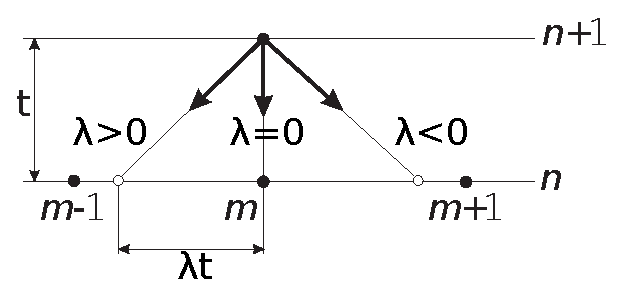
\includegraphics[width=0.5\textwidth]{png/gcm-idea.eps}}
	\caption{Основная идея сеточно-характеристического метода}
	\label{pic:gcm-idea}
\end{figure}
Сформулируем алгоритм одного шага метода по времени (см. \ref{pic:gcm-idea}):
\begin{enumerate}
	\item Из узлов сетки на новом временном слое выпускаются характеристики на предыдущий слой. Количество характеристик равно количеству переменных в системе.
	\item В точках пересечения характеристик с предыдущим слоем вычисляются значения функции и пересчитываются в инварианты Римана.
	\item Инварианты Римана переносятся на новый слой, производится их пересчёт в значения функции.
\end{enumerate}

Описанный выше метод применим только в тех случаях, если точка пересечения выпущенной из расчётного узла характеристики и предыдущего временного слоя не выходит за пределы области интегрирования. Это условие может быть нарушено в нескольких случаях (см. \ref{pic:outer-cases}). Во-первых, в случае граничных узлов, когда направление характеристики вне тела -- точка номер 2. Во-вторых, в случае внутренних узлов, когда характеристика пересекает границу тела до пересечения с предыдущим временным слоем -- точка номер 1. Такая же ситуация возможна и для граничных узлов при наличии острых углов у области интегрирования -- точка номер 3. Рассмотрим каждый из этих случаев по отдельности.
\begin{figure}[H]
	\center{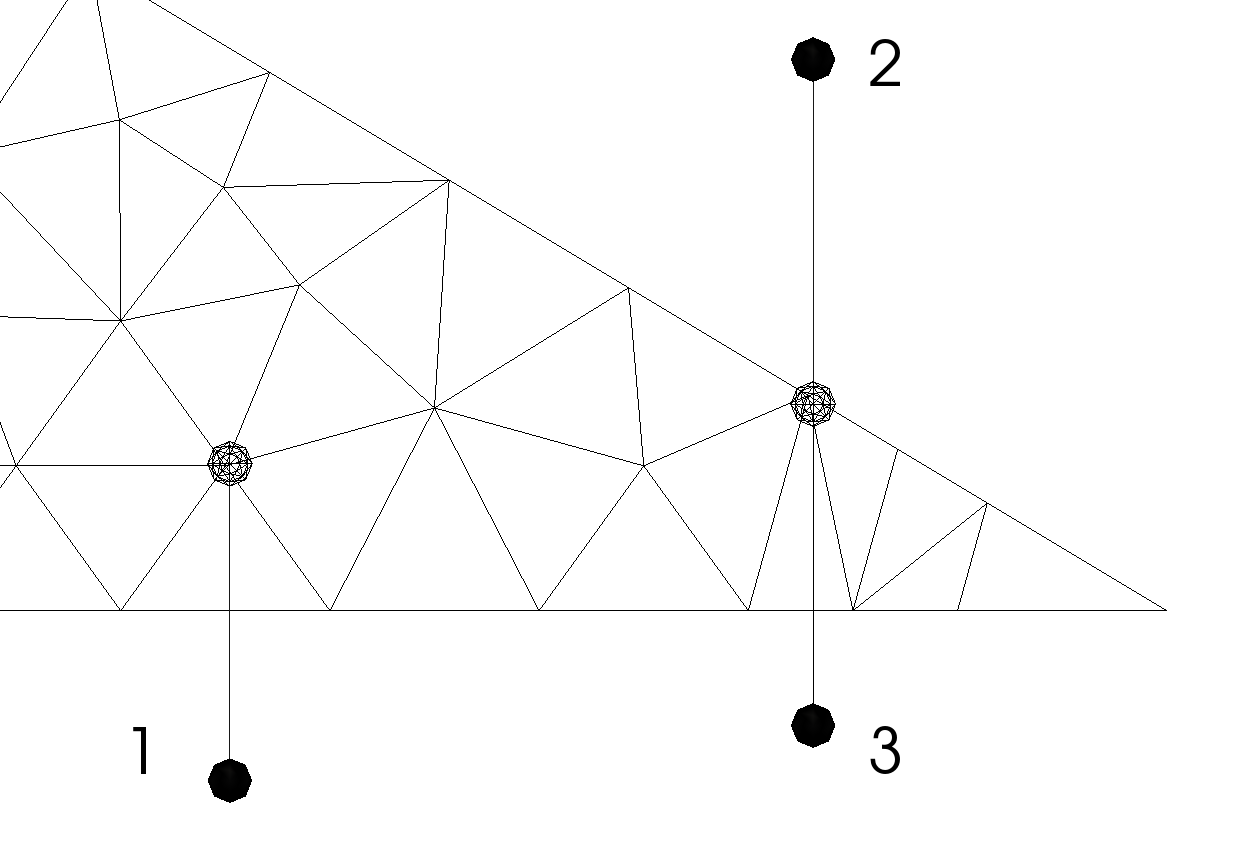
\includegraphics[width=0.8\textwidth]{png/outer-cases.png}}
	\caption{Тело с острым углом на границе. Различные случаи выпадения характеристик за область интегрирования}
	\label{pic:outer-cases}
\end{figure}


\subsubsection{Расчёт граничных узлов}
В \cite{chelnokov} был предложен следующий алгоритм расчёта граничных условий. Сначала вычисления проводятся только для внутренних характеристик -- значения инвариантов Римана, соответствующие выпавшим за пределы области характеристикам, зануляются. Затем применяется граничный корректор, цель которого -- обеспечить выполнение заданных граничных условий.

Запишем общий вид линейного граничного условия:
\begin{equation}
	\label{general_border_condition}
	\mathbf{B} \vec{u} = \vec{b}.
\end{equation}

К примеру, для заданной на границе скорости:
\begin{align}
\mathbf{B} =
\left( \begin{array}{cccccccccccc}
1 & 0 & 0 & 0 & 0 & 0 & 0 & 0 & 0 \\ 
0 & 1 & 0 & 0 & 0 & 0 & 0 & 0 & 0 \\ 
0 & 0 & 1 & 0 & 0 & 0 & 0 & 0 & 0 \\ 
\end{array} \right),
\end{align}

\begin{equation}
	\vec{b} = \left( v_{\xi}, v_{\eta}, v_{\zeta} \right)^T,
\end{equation}
где $ v_{\xi} v_{\eta} v_{\zeta}$ -- компоненты скорости в локальном базисе, связанном с границей тела.

Для заданной на границе внешней силы:
\begin{align}
\mathbf{B} =
\left( \begin{array}{cccccccccccc}
0 & 0 & 0 & n_x & n_y & n_z & 0 & 0 & 0 \\ 
0 & 0 & 0 & 0 & n_x & 0 & n_y & n_z & 0 \\ 
0 & 0 & 0 & 0 & 0 & n_x & 0 & n_y & n_z \\ 
\end{array} \right),
\end{align}
где $\vec{n}$ -- единичная нормаль к поверхности в точке задания условия.

\begin{equation}
	\vec{b} = \left( \sigma_{\xi \zeta}, \sigma_{\eta \zeta}, \sigma_{\zeta \zeta} \right)^T,
\end{equation}
где $\sigma_{\xi \zeta}, \sigma_{\eta \zeta}, \sigma_{\zeta \zeta}$ -- компоненты тензора напряжений в локальном базисе, связанном с границей тела.

Составим из собственных векторов, соответствующих внешним собственным значениям, матрицу $\mathbf{\Omega^{*}}$. Будем искать решение на новом слое $\vec{u}^{n+1},$ удовлетворяющее граничным условиям, в виде
\begin{equation}
	\vec{u}^{n+1} = \vec{u}^{*} + \mathbf{\Omega^{*}} \vec{\alpha},
\end{equation}
где $\alpha$ -- неизвестный пока вектор, $\vec{u}^{*}$ -- решение, полученное на этапе внутреннего расчёта. Тогда для $\vec{\alpha}$ получаем СЛАУ:
\begin{equation}
\label{border_slau}
	\left( \mathbf{B} \mathbf{\Omega*} \right) \vec{\alpha} = \vec{b} -  \mathbf{B} \vec{u}^{*}.
\end{equation}
Такой подход означает вычисление внешних инвариантов Римана из условия выполнения заданных соотношений на границе. Другими словами, мы подбираем линейную комбинацию "пришедших извне"\space{} волн так, чтобы выполнялось граничное условие.
Невырожденность системы \eqref{border_slau} равносильна корректности заданных граничных условий.


\subsubsection{Расчёт внутренних узлов с внешними характеристиками}
Для возможности расчёта случаев, изображённых под номером 1 на рис. \ref{pic:outer-cases}, в \cite{magomedov_kholodov_1988} предложен следующий способ. При выполнении  очередного шага по времени сначала производится расчёт всех граничных узлов. После чего для внутренних узлов с выпавшими за пределы тела характеристиками интерполяция внешних инвариантов Римана производится не по предыдущему временному слою, а по границе тела. Точка, в которой проводится интерполяция, находится между двумя слоями во времени. Такой подход корректен, так как значения на границе на новом временном слое уже посчитаны.

Оставшийся случай под номером 3 мог бы быть выполнен аналогично предыдущему, но при расчёте граничных узлов нельзя проводить интерполяцию во времени, так как нет гарантии, что область интерполяции уже была рассчитана на новом временном слое. Поэтому следует сначала определить значение в точке пересечения характеристики с границей, посчитав в этой точке значение функции как для любого другого граничного узла. Таких "переотражений"\space{} может быть несколько.

Вообще стоит отметить, что сложные случаи при расчёте границы области интегрирования -- определяющая проблема при реализации сеточно\hyp{}характеристического метода на неструктурированных расчётных сетках.



\subsubsection{Расчёт граничных узлов и узлов с внешними характеристиками на структурированной расчётной сетке}
Изложенный выше алгоритм расчёта граничных случаев актуален для неструктурированных расчётных сеток. Для регулярных сеток можно использовать более простой метод фиктивных внешних узлов. Его основная идея -- введение вдоль границ тела вспомогательных расчётных узлов, значения в которых выставляются так, чтобы при сквозном счёте границы  автоматически выполнялись поставленные условия. 

Допустим, вдоль границы, перпендикулярной оси $x$, поставлено условие фиксированной внешней силы
\begin{equation}
	\sigma_{xx} = S_{xx}, \sigma_{xy} = S_{xy}, \sigma_{xz} = S_{xz}.
\end{equation}
Пусть вдоль рассматриваемой оси граничный узел имеет индекс 0, тогда внутренние узлы имеют положительные индексы, а фиктивные узлы -- отрицательные. Перед очередной ступенью расчёта вдоль данной оси выставим во вспомогательных узлах следующие значения:

\begin{eqnarray}
	{\sigma_{xx}}_{(-i)} = -{\sigma_{xx}}_{(i)} + 2S_{xx}, \\
	{\sigma_{xy}}_{(-i)} = -{\sigma_{xy}}_{(i)} + 2S_{xy}, \\
	{\sigma_{xz}}_{(-i)} = -{\sigma_{xz}}_{(i)} + 2S_{xz}, \\
	{v_x}_{(-i)} = {v_x}_{(i)}, \\
	{v_y}_{(-i)} = {v_y}_{(i)}. \\
	{v_z}_{(-i)} = {v_z}_{(i)}.
\end{eqnarray}

Значения для $ \sigma_{yy}, \sigma_{yz}, \sigma_{zz} $ ставить не требуется, так как они не участвуют в данной ступени расчёта. Далее будем считать граничные узлы таким же образом, как и внутренние. Полученное решение будет удовлетворять поставленным граничным условиям с первым порядком точности. 

Это можно объяснить из следующих соображений. Если провести прямую, соответствующую линейной интерполяции для компонент тензора напряжения, через $(i)$-й и $(-i)$-й узлы, то её значение в нулевом узле совпадёт граничным условием. Аналогично для компонент скорости, которые не должны меняться в граничных узлах при условии фиксированной поверхностной силы.

Вводя достаточное количество фиктивных узлов, добиваемся того, что все характеристики попадают внутрь расчётной области.

Метод фиктивных узлов удобен ещё тем, что он отлично согласуется с реализацией параллельных расчётов с раздельной памятью -- через эти узлы принимается информация от соседних процессов, необходимая для продолжения расчётов.


\subsection{Интерполяция в задачах сеточно\hyp{}характеристического метода}
\subsubsection{Общие замечания}
Из вышесказанного следует, что для реализации сеточно\hyp{}характеристического метода необходимо производить интерполяцию значений функции в пространстве между узлами сетки. Порядок интерполяции определяет порядок метода по пространству. 

Как правило, интерполяция проводится в два этапа: сначала полиномом некоторой степени приближается значение функции в искомой точке, затем полученное значение корректируется для устранения нефизичных осцилляций, возникающих в схемах порядка выше первого. Корректировка сводится к применению ограничителя -- "лимитера"\space{} на полученное значение. Наиболее простой и распространённый вариант -- так называемый "minmax"\space{}лимитер, который контролирует минимальное и максимальное значения результата интерполяции исходя из значений функции в соседних точках. Другой пример -- когда при возникновении осцилляций в данной точке порядок интерполяции понижается до первого. Это так называемые гибридные схемы.

В данной работе используется "minmax"\space{}лимитер, так как с ним волновые фронты меньше подвержены сглаживанию, что является важным в задачах моделирования неразрушающего контроля.

\subsubsection{Интерполяция на структурированной расчётной сетке}
В случае структурированной сетки и расщепления по направлениям независимо от размерности решаемой задачи интерполяция производится не в пространстве, а на прямой, вдоль которой выполняется ступень расчёта. Это значительно упрощает задачу. Существует множество способов интерполяции функции по исходным данным, распределённым на прямой. 

В данной работе было решено воспользоваться интерполяционными полиномами в форме Ньютона \cite{petrov_lobanov}. Пусть известны значения функции $f(t)$ в точках $t_i$.
Определим конечные разности порядка $k$ для $i$-й точки как 
\begin{eqnarray}
\label{newton_finite_diff}
f(t_i, t_{i+1}, ..., t_{i+k}) = \frac{f(t_{i+1}, ..., t_{i+k}) - f(t_i, ..., t_{i+k-1})}{t_{i+k} - t_{i}}, \\
f(t_i, t_{i+1}) = \frac{f(t_{i+1}) - f(t_i)}{t_{i+1} - t_i}.
\end{eqnarray}
Тогда аппроксимационный полином степени $n$
\begin{equation}
\label{newton_polynom}
N_n(t) = f(t_1) + f(t_1, t_2)(t-t_1) + ... + f(t_1, ..., t_{n+1})(t-t_1)...(t-t_n).
\end{equation}

Пусть точки с известными значениями функции расположены на одинаковых расстояниях $\Delta t$ друг от друга, а точка поиска -- на расстоянии $q \Delta t$ от первой из них. Пусть известные значения записаны в массив данных (нумерация с нуля). Тогда после некоторых упрощений формул \eqref{newton_finite_diff} и \eqref{newton_polynom} получим компактный алгоритм нахождения значения в точке поиска с порядком точности $n$ (значения в массиве в ходе работы алгоритма будут перезаписаны!):


%\begin{minipage}{\linewidth}
\begin{lstlisting}
result = f[0];
for (int i = 1; i <= n; i++) {
	for (int j = 0; j < n - i + 1; j++) {
		f[j] = (f[j + 1] - f[j]) * ((q - i + 1) / i);
	}
	result += f[0];
}
\end{lstlisting}
%\end{minipage}
Теоретически, получен алгоритм интерполяции произвольного порядка на структурированной сетке. На практике такой подход сталкивается с двумя трудностями. 

Во-первых, необходимо специально исследовать устойчивость такого рода схем. Как было показано в \cite{favorskaya_disser}, наглядное правило Куранта (метод устойчив, если значение интерполируется в области зависимости решения) не всегда применимо в этом случае. Например, интерполяции третьего порядка с шаблоном, изображённым на рис. \ref{pic:stability}, устойчива при числе Куранта от 1 до 2. Из правила Куранта следовала бы устойчивость от 0 до 3.

\begin{figure}[H]
	\center{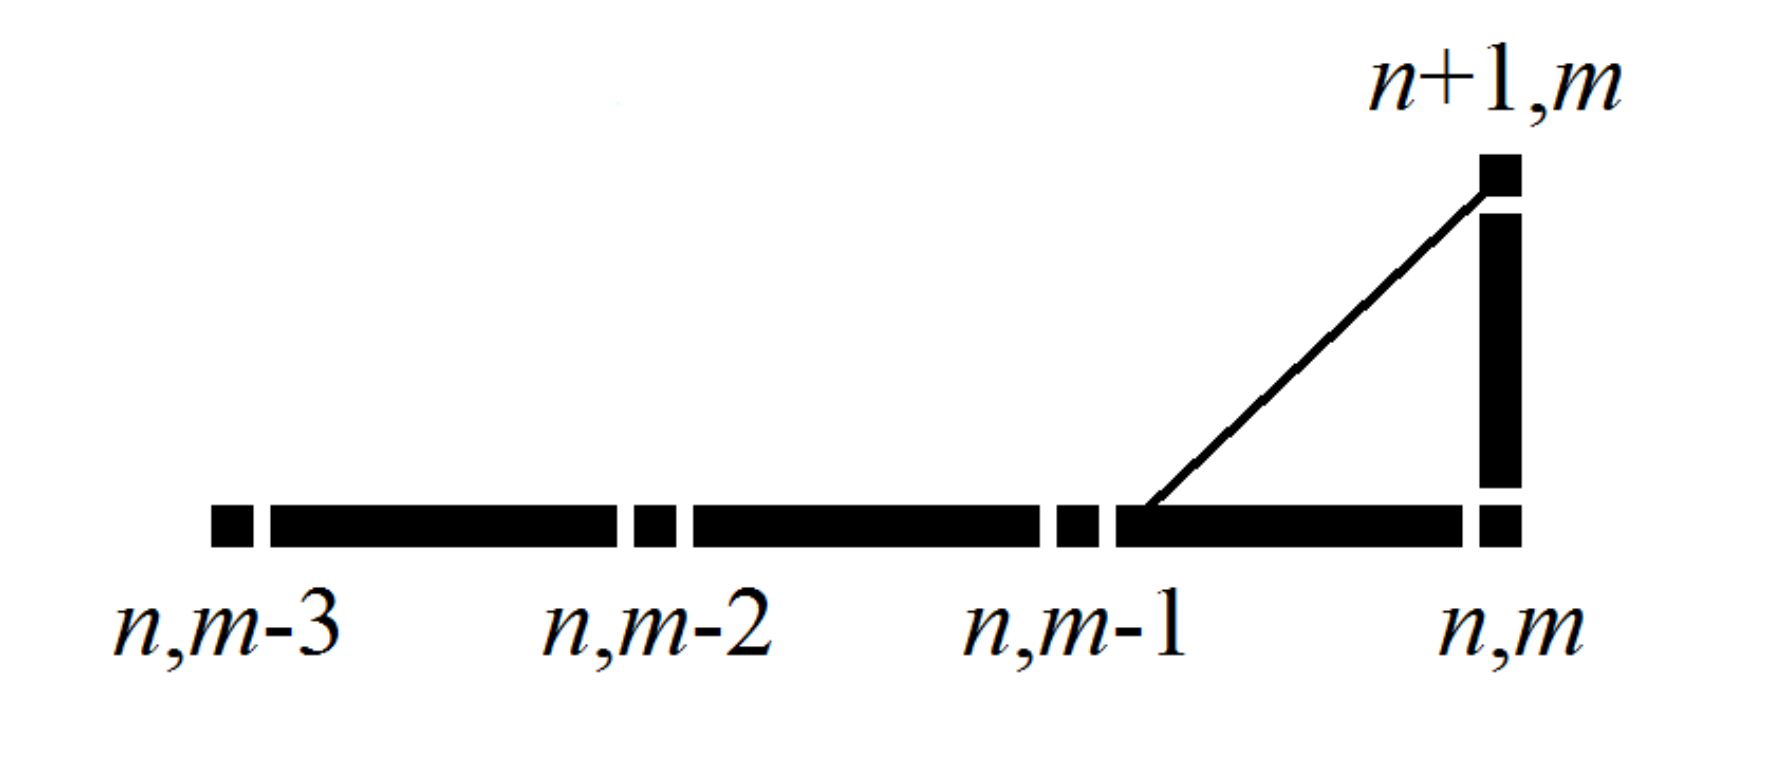
\includegraphics[width=0.5\textwidth]{png/stability.png}}
	\caption{Четырёхточечный шаблон для расчёта третьего порядка аппроксимации}
	\label{pic:stability}
\end{figure}

Во-вторых, при использовании метода фиктивных узлов с увеличением порядка схемы развивается неустойчивость на границе. Это связано с фактической экстраполяцией значений во вспомогательных узлах -- нарушение уже названного правила Куранта.


\subsubsection{Интерполяция на неструктурированной расчётной сетке}
В случае неструктурированной расчётной сетки необходимо производить интерполяцию в пространстве той размерности, в какой решается задача. Далее рассматриваются только сетки на триангуляциях -- треугольная в двумерном случае и тетраэдрическая в трёхмерном.

Большинство известных автору работ используют метод интерполяции, предложенный в \cite{chelnokov_agapov}. Он заключается во введении на рёбрах треугольника (тетраэдра) дополнительных расчётных узлов, с помощью которых повышается порядок аппроксимации. На рис. \ref{pic:triangle-interp} показана интерполяция второго порядка в тетраэдре -- по одному дополнительному узлу на каждом ребре тетраэдра.

\begin{figure}[H]
	\center{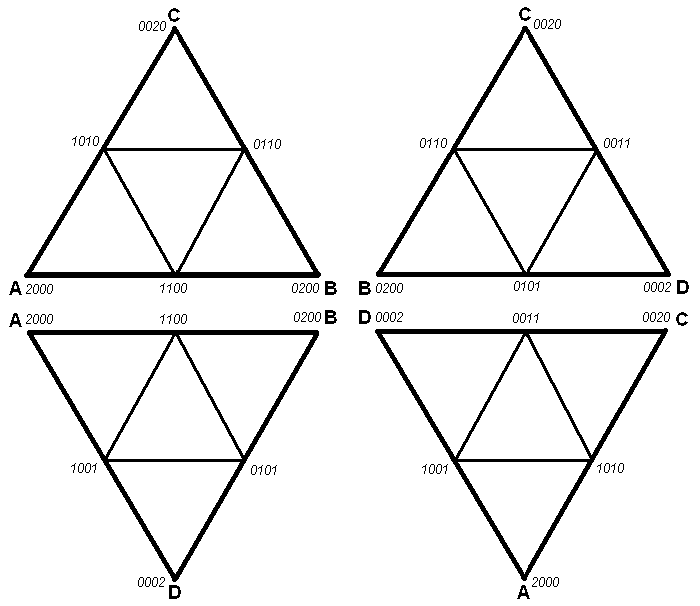
\includegraphics[width=0.5\textwidth]{png/triangle-interp.png}}
	\caption{Интерполяция в тетраэдре методом вспомогательных узлов на рёбрах}
	\label{pic:triangle-interp}
\end{figure}

К достоинствам этого метода следует в первую очередь отнести возможность реализации интерполяции произвольного порядка. К недостаткам - рост числа расчётных узлов и усложнение геометрии сетки. Последнее может быть критичным в задачах с большими деформациями.

В данной работе предложен альтернативный подход, позволяющий осуществить интерполяцию первого и второго порядка без введения вспомогательных узлов. Далее будем говорить о треугольниках, для тетраэдров всё аналогично. 

Пусть известны значения функции $f$ в вершинах треугольника $\vec{a}, \vec{b}, \vec{c}$ и необходимо определить её значение в некоторой точке $\vec{q}$. Введём барицентрические координаты $\lambda_i$ из условия 
\begin{eqnarray}
\vec{q} = \lambda_0 \vec{a} + \lambda_1 \vec{b} + \lambda_2 \vec{c}, \\
\lambda_0 + \lambda_1 + \lambda_2  = 1
\end{eqnarray}
Физический смысл $\lambda$ таков: если расположить в точках $\vec{a}, \vec{b}, \vec{c}$ массы $\lambda_0, \lambda_1, \lambda_2$ соответственно, то центр масс такой системы будет в точке $\vec{q}$. 

Ещё более полезен их геометрический смысл, показанный на рис. \ref{pic:barycentric}. К примеру, условие попадания точки внутрь треугольника -- положительность всех её барицентрических координат, условие нахождения точки во внутренности угла $\angle a b c$ будет $\lambda_1 < 1, \lambda_0 > 0, \lambda_2 > 0$. Эти свойства ещё более полезны в трёхмерном пространстве, когда изобразить задачу на листе бумаги становится сложнее.

\begin{figure}[H]
	\center{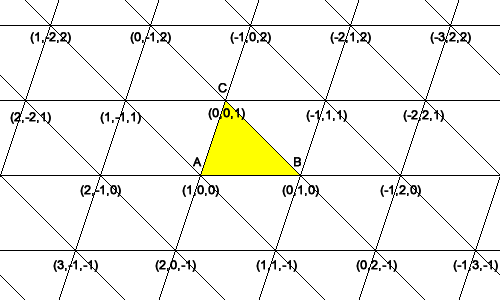
\includegraphics[width=1.0\textwidth]{png/barycentric.png}}
	\caption{Геометрический смысл барицентрических координат}
	\label{pic:barycentric}
\end{figure}

Итак, если известны значения функции $f$ в точках треугольника $\vec{p}_i$, составим следующий интерполяционный многочлен:
\begin{equation}
P(\vec{x}) = \sum_{i} \lambda_i(\vec{x}) f(\vec{p}_i).
\end{equation}
Здесь $\lambda_i(\vec{x})$ -- барицентрические координаты произвольной точки $\vec{x}$ в этом треугольнике. Такой многочлен в точности воспроизводит линейную функцию: пусть
\begin{equation}
z(\vec{x}) = a + \vec{b} \vec{x},
\end{equation}
тогда
\begin{equation}
P(\vec{x}) = \sum_{i} \lambda_i({\vec{x}}) (a + \vec{b} \vec{p}_i) = a \sum_{i} \lambda_i(x) + \vec{b} \sum_{i} \lambda_i(x) \vec{p}_i = a + \vec{b} \vec{x} = z(\vec{x}).
\end{equation}

Если в точках треугольника $\vec{p}_i$ известны ещё и значения градиента $\nabla f = \vec{g}$, составим интерполяционный многочлен, в точности воспроизводящий квадратичную функцию:
\begin{equation}
P(\vec{x}) = \sum_{i} \lambda_i(\vec{x}) \Big(f(\vec{p}_i) + \frac{1}{2} {\vec{g}_i}^T (\vec{x} - \vec{p}_i) \Big).
\end{equation}
Доказательство:
\begin{align}
z(\vec{x}) = \vec{x}^T \mathbf{A} \vec{x} + \vec{b} \vec{x} + c, \\
g(\vec{x}) = \nabla z(\vec{x}) = 2 \mathbf{A} \vec{x} + \vec{b}, \\
P(\vec{x}) = \sum_{i} \lambda_i({\vec{x}}) \Big( {\vec{p}_i}^T \mathbf{A} \vec{p}_i + \vec{b} \vec{p}_i + c + \frac{1}{2} (2\mathbf{A}\vec{p}_i + \vec{b})^T (\vec{x} - \vec{p}_i) \Big) = \\
\sum_{i} \lambda_i({\vec{x}}) \Big( {\vec{p}_i}^T \mathbf{A} \vec{p}_i + \vec{b} \vec{p}_i + c + {\vec{p}_i}^T \mathbf{A} \vec{x} + \frac{1}{2} \vec{b}\vec{x} - {\vec{p}_i}^T \mathbf{A} \vec{p}_i - \frac{1}{2} \vec{b} \vec{p}_i  \Big) = \\
\sum_{i} \lambda_i({\vec{x}}) \Big( {\vec{p}_i}^T \mathbf{A} \vec{x} + \frac{1}{2} \vec{b} \vec{p}_i + c + \frac{1}{2} \vec{b}\vec{x}  \Big) = \\
\vec{x}^T \mathbf{A} \vec{x} + \vec{b} \vec{x} + c = z(\vec{x}).
\end{align}

Идея построения многочлена взята из \cite{cgal_interpolation}, где такого же рода интерполяционные многочлены применяются для аппроксимации на разбиениях Вороного (так называемый метод естественных соседей \cite{sibson, natural_neighbors}).

Ограничение изложенного метода в том, что он не допускает обобщения уже на случай третьего порядка точности. Это следствие, как минимум, того, что в интерполяционном многочлене используется всего 3 (4 в трёхмерном случае) свободных параметра, и то, что возможна реализация второго порядка -- уже большая удача. Попытка использовать больше свободных параметров требует наличия известных производных на один порядок выше, чем в данном случае, что в любом случае должно сильно ухудшить свойства интерполяции.


\subsubsection{Численное дифференцирование на неструктурированной расчётной сетке}
Как ясно из предыдущего параграфа, для возможности интерполяции второго порядка без вспомогательных узлов необходимо знание градиента интерполируемой функции. В этой связи предлагается перед выполнением очередной ступени расчёта вычислять градиент решения на текущем временном слое. Будучи один раз вычислено для каждого узла сетки, значение градиента потом используется множество раз при интерполяции различных точек.

Реализованный в данной работе метод численного дифференцирования был, по-видимому, впервые предложен в \cite{sibson}. Для вычисления градиента в некотором узле сетки находятся все ближайшие узлы-соседи, для которых выполнено (см. рис. \ref{pic:gradient}):
\begin{equation}
f_i - f^{*} = \nabla f (\vec{x}_i - \vec{x}^{*}) + O( \lVert \vec{x}_i - \vec{x}^{*} \rVert ^2)
\end{equation}
\begin{figure}[H]
	\center{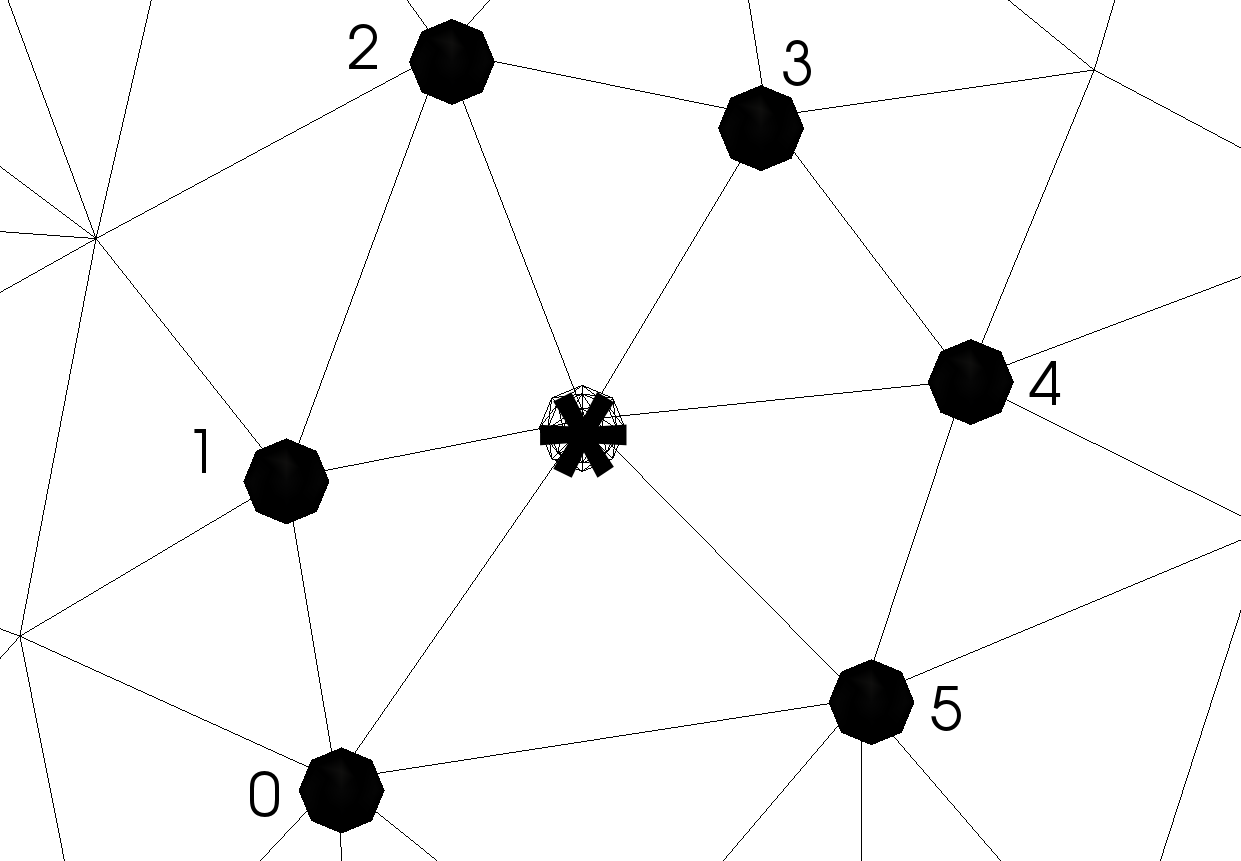
\includegraphics[width=0.7\textwidth]{png/gradient.png}}
	\caption{К пояснению метода численного дифференцирования}
	\label{pic:gradient}
\end{figure}
Записывая это уравнение для всех узлов-соседей, получаем переобусловленную СЛАУ на значения градиента:
\begin{eqnarray}
\mathbf{A}\vec{g} = \vec{b}, \\
\mathbf{A}_{ij} = (\vec{x}_i - \vec{x}^{*})_j, \\
b_i = f_i - f^{*}.
\end{eqnarray}
СЛАУ решается методом наименьших квадратов \cite{petrov_lobanov} с весами, равными расстояниям от рассчитываемого узла до соответствующего соседа:
\begin{eqnarray}
\Big( \mathbf{A}^T \mathbf{W} \mathbf{A} \Big) \vec{g} = \Big( \mathbf{A}^T \mathbf{W} \Big) \vec{b}, \\
\mathbf{W}_{ij} = \lVert x_i - x^{*} \rVert,\ i = j, \\
\mathbf{W}_{ij} = 0, \ i \neq j.
\end{eqnarray}

Характерная размерность матрицы $\mathbf{A}$ в двумерном случае -- $6\times2$, в трёхмерном случае -- $15\times3$ (рис. \ref{pic:num_neighbors}), то есть система хорошо обусловлена.
\begin{figure}[H]
	\center{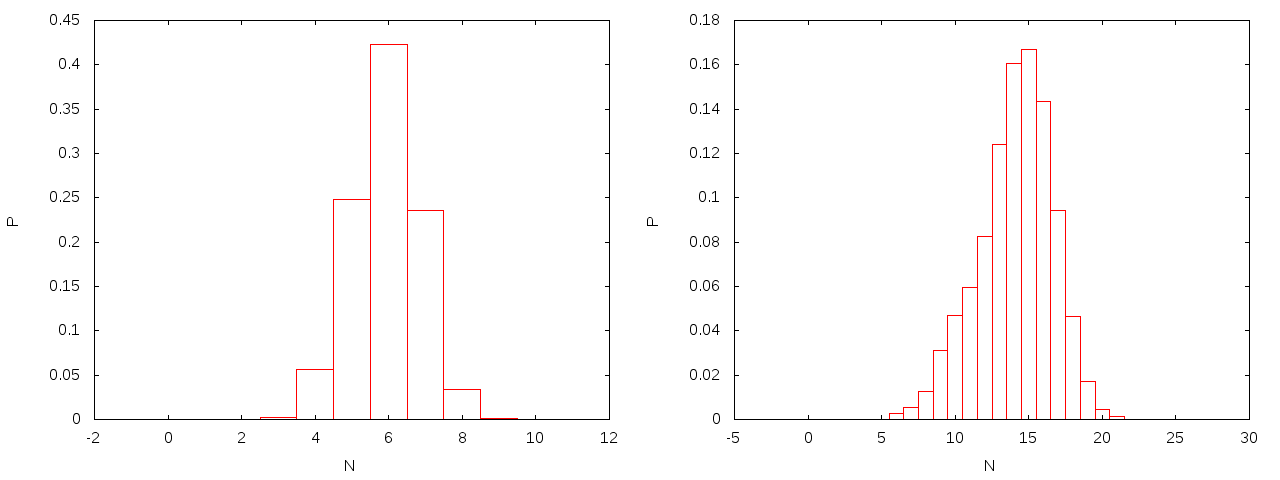
\includegraphics[width=1\textwidth]{png/num-neighbors.png}}
	\caption{Гистограммы числа соседних вершин в двумерном и трёхмерном случаях}
	\label{pic:num_neighbors}
\end{figure}


\subsection{Задача поиска ячейки сетки, содержащей точку пересечения характеристики с предыдущим временным слоем}
Для того, чтобы произвести интерполяцию на неструктурированной сетке, необходимо найти треугольник (тетраэдр), который содержит точку интерполяции. Задача обычного поиска содержащей точку ячейки в триангуляции имеет множество решений. Их можно разделить на два подхода. Первый -- хранить триангуляцию в специальной структуре быстрого поиска, которая позволяет за логарифмическое время находить указанную точку в триангуляции. Второй -- хранить триангуляцию в виде, в котором каждая ячейка имеет указатели на своих ячеек-соседей (3 в двумерном и 4 в трёхмерном случае) и осуществлять поиск переходом от ячейки к ячейке, выбирая правильное в некотором смысле направление.

Однако задача нахождения ячейки, содержащей точку пересечения характеристики с предыдущим временным слоем в сеточно\hyp{}характеристическом методе, имеет нюансы, которые не позволяют полностью свести её к выше описанной. Это иллюстрирует рис. \ref{pic:locate_cell}. Случай под номером 1 -- пример, когда задачи поиска эквивалентны. Случай под номером два -- случай внешней характеристики у внутреннего узла -- требует нахождения точки пересечения характеристики с границей области интегрирования. Случай номер 3 -- ситуация, когда применение обычного алгоритма даёт неверный результат.

Отсюда можно сделать вывод, что алгоритм поиска требует модификации по сравнению с его обычной реализацией. В данной работе решено было использовать стратегию поиска вдоль линии -- "line walk" \cite{line_walker}. Она относится ко второй из названных выше групп подходов и наиболее естественно учитывает запросы сеточно-характеристического метода. 

\begin{figure}%[H]
	\center{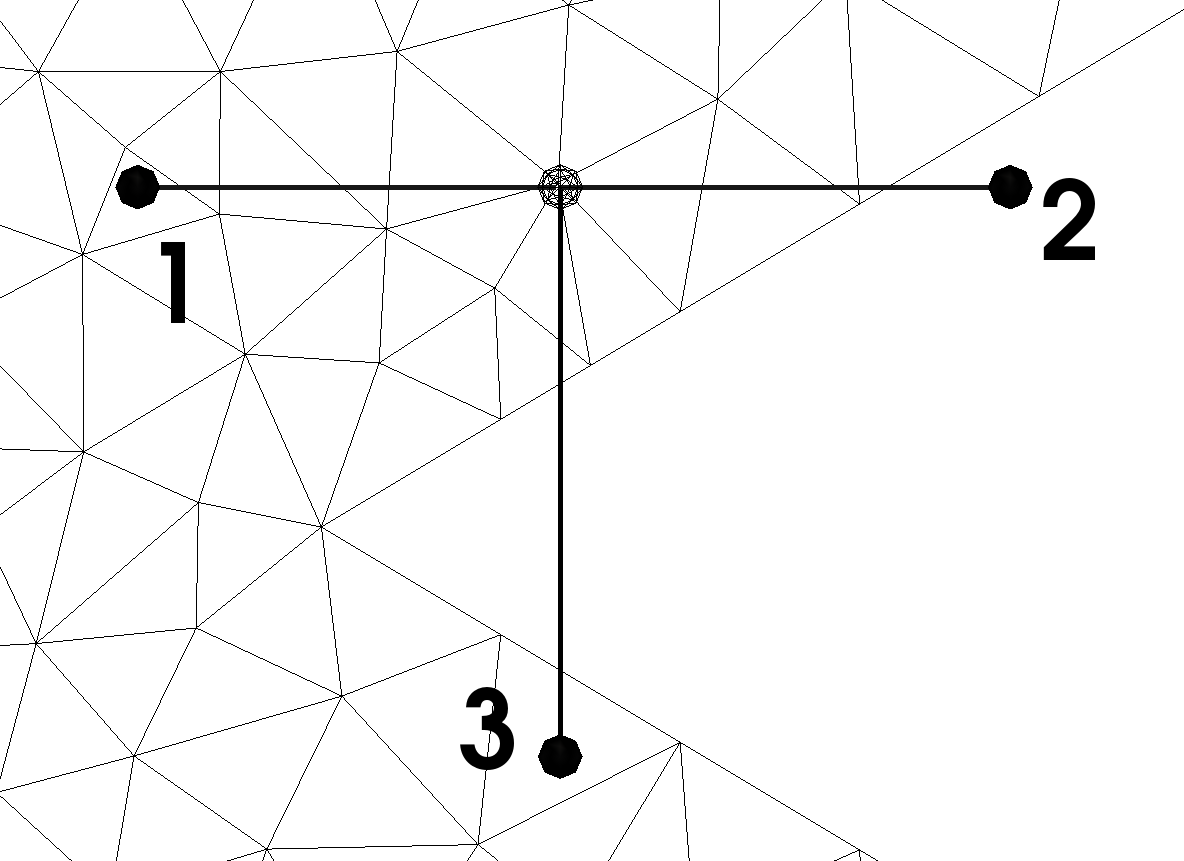
\includegraphics[width=0.5\textwidth]{png/locate_cell.png}}
	\caption{Случаи поиска}
	\label{pic:locate_cell}
\end{figure}

Введём 
\begin{equation}
orientation(a, b, c) = \det{\begin{vmatrix}b_x - a_x & c_x - a_x \\
                                           b_y - a_y & c_y - a_y \end{vmatrix}} -
\end{equation}
-- ориентированную площадь треугольника $a, b, c$.

\begin{figure}
	\center{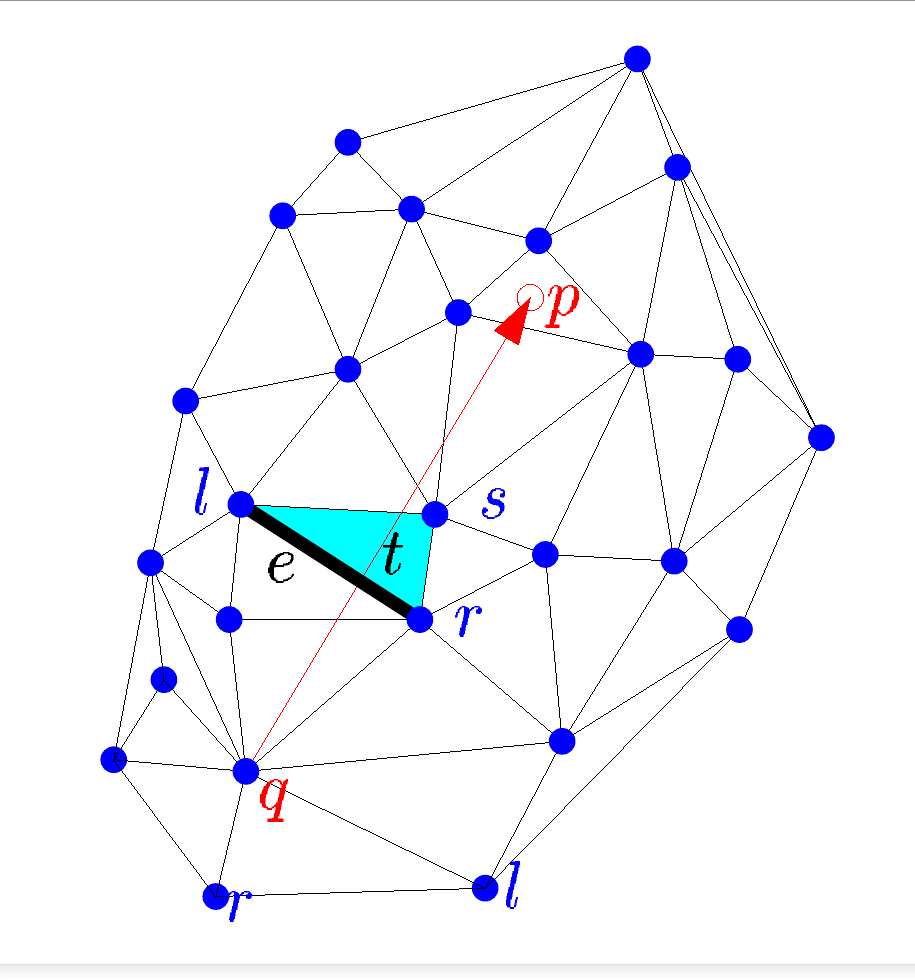
\includegraphics[width=0.5\textwidth]{png/line-walk.png}}
	\caption{Поиск вдоль линии в триангуляции \cite{line_walker}}
	\label{pic:line-walk}
\end{figure}

Для простоты в двумерном случае (трёхмерный случай рассматривается аналогично) опишем основные стадии алгоритма поиска точки по линии (рис. \ref{pic:line-walk}):
\begin{itemize}
\item Имеем исходную вершину $q$ в триангуляции и точку для поиска $p$
\item Рассматриваем все ячейки, имеющие исходную вершину, и выбираем среди них ту, которая содержит внутри себя луч $qp$. Это делается, например, на основе анализа барицентрических координат точки $p$ в каждой ячейке -- см. \ref{pic:barycentric}
\item Обозначим вершину найденной ячейки, лежащую слева от $qp$, как $l$, вершину, лежащую справа, как $r$ и вершину $s = q$
\item Выполнено $orientation(s, r, l) > 0$
\item Далее до тех пор, пока $orientation(p, r, l) < 0$, повторяем:
	\begin{itemize}
		\item Переходим в ячейку, разделяющую с текущей точки $r, l$
		\item Переносим вершину $s$ в новую ячейку на свободное от $r, l$ место
		\item Если $orientation(s, q, p) < 0$, $r = s$, иначе $l = s$
	\end{itemize}
\item Ячейка, содержащая $p$, найдена
\end{itemize}

Простота написанного алгоритма обманчива. В нём не было рассмотрено случаев наподобие $orientation(s, q, p) = 0$. Реализация стабильного поиска, учитывающего все предельные ситуации в двумерном пространстве сложна, а в трёхмерном -- не факт, что возможна. Между тем, предельные случаи имеют место быть, например, вдоль координатных осей при расчёте фигур правильной формы, когда направления расчёта также совпадают с этими осями. По-видимому, наиболее простой выход из этой ситуации -- отказаться от проведения ступеней расчёта вдоль координатных осей.

Между тем, данный метод имеет большое преимущество в решении всех проблем, изображённых на рис. \ref{pic:locate_cell}, а также позволит корректировать наклон характеристики в зависимости от реологии ячеек при расчёте неоднородных материалов.

















